\documentclass{beamer}
\usepackage[utf8]{inputenc}
\usepackage{hyperref} 
\usepackage{pgfpages}
\usepackage{amsmath,amssymb,mathrsfs}
\setbeamertemplate{navigation symbols}{} % turns off navigation symbols at the bottom of slides
\usepackage{graphicx}
\usepackage{amsmath}
\usepackage{caption}
\usepackage{subcaption}
\usepackage[round]{natbib}

\newcommand{\ubar}[1]{\underaccent{\bar}{#1}}
\newcommand{\p}{\prime}
\newcommand{\ev}{\mathbb{E}}
\newcommand{\lagr}{\mathcal{L}}
\newcommand{\inv}[1]{#1^{-1}}
\newcommand{\R}{{\rm I\!R}}
\newcommand{\U}{\mathcal{U}}
\renewcommand{\H}{\mathcal{H}}
\newcommand{\pderiv}[2]{\frac{\partial#1}{\partial #2}}

\title{Optimal Taxation with Heterogeneous Rates of Return}
\author[Hoffman, Shourideh]
{Nick Hoffman\inst{1} \and Ali Shourideh \inst{1}}
\institute[ ] 
{\inst{1} Carnegie Mellon University}

\begin{document}
    \begin{frame}
        \titlepage 
    \end{frame}

% \begin{frame}
%     \frametitle{}
%     \tableofcontents
% \end{frame}

\section{Introduction}
\begin{frame}
    \frametitle{Summary}

    \begin{itemize}
        \item Study optimal \textit{nonlinear} taxation in an economy where agents are heterogeneous in the (stochastic) returns to their investment
        \item Static model
        \begin{itemize}
            \item Risky investment is susbidized according to a nonlinear function of return
            \item Wedge on risk-free savings of productive entrepreneurs is positive, increasing in return
        \end{itemize}
        \item Dynamic model
        \begin{itemize}
            \item IID case: optimal wedges are independent of history
        \end{itemize} 
        \item Implementation
        \begin{itemize}
            \item In progress: how to implement constrained-efficient allocations with taxes and transfers?
        \end{itemize}
    \end{itemize}

\end{frame}

\begin{frame}
    \frametitle{Motivation}

    \begin{itemize}
        \item US distribution of wealth exhibits thick (Pareto) tails
        \begin{itemize}
            \item \cite{benhabib2011distribution}: the heavy tail is generated by capital, rather than labor, income risk 
            \item Tail populated by entrepreneurs, investors, business owners
            \item Need to understand optimal taxation of those whose income derives from investment, rather than labor effort
        \end{itemize} % which motivates
        \item Capital income, wealth taxation have been topics of debate
        \begin{itemize}
            \item \cite{saez2019triumph}: argue for wealth taxation 
            \item This introduces obvious disincentives to invest 
            \item Mirrlees: framework in which to study the optimal tradeoff between \textit{redistribution} and \textit{efficiency} 
        \end{itemize}
    \end{itemize}

\end{frame}

\begin{frame}
    \frametitle{Related Literature}

    \begin{itemize}
        \item Static Mirrleesian taxation: \cite{mirrlees1971exploration}, \cite{diamond1998optimal}, \cite{saez2001using}
        \begin{itemize}
            \item Government can set arbitrarily nonlinear taxes, subject to informational frictions
        \end{itemize}
        \item Dynamic extensions: \cite{golosov2003optimal}, \cite{kocherlakota2005zero}, \cite{albanesi2006dynamic}
        \begin{itemize}
            \item Possibility of a positive optimal wedge on savings
            \item Intertemporal return constant across the population
        \end{itemize}
        \item Heterogeneous returns: \cite{shourideh2014optimal}, \cite{phelan2019business}, \cite{phelan2019differential}
    \end{itemize}

\end{frame}

\section{Static Model}
\begin{frame}
    \frametitle{Static Model: Agents, Assets, and Production}

    \begin{itemize}
        \item Continuum of agents, \( i\in[0,1] \)
        \item Two periods, \( t = 0,1 \)
        \item Agents have privately-known type \( \theta\in\Theta=\left[\underline{\theta},\overline{\theta}\right] \)
        \begin{itemize}
            \item Distributed according to differentiable CDF \( F\left( \theta \right) \)
        \end{itemize}
        \item Two assets 
        \begin{itemize}
            \item Risk-free savings bond: zero net supply, return \( R \)
            \item Risky entrepreneurial endeavor: stochastic return \( \theta \)
        \end{itemize} 
        \item Initial endowment \( w \)
        \item Output: an agent of type \( \theta \) who invests \( k \) into risky technology produces 
        \begin{equation}
            y = \begin{cases}
                \theta k & \text{with probability }\alpha \\
                0 & \text{with probability }1 - \alpha
            \end{cases}
        \end{equation}
    \end{itemize}

\end{frame}

\begin{frame}
    \frametitle{Static Model: Taxes}
    
    Government
    \begin{itemize}
        \item Observes incomes \( y \) and \( Rb \), but not \( \theta \) or \( k \)
        \item Levies taxes according to tax function \( T\left( y,Rb \right) \)
        \item Mirrleesian problem: must set \( T \) to maximize total utility, subject to the constraint that \( T \) cannot induce individuals to invest a ``suboptimal'' amount
    \end{itemize}

\end{frame}

\begin{frame}
    \frametitle{Static Model: Taxes}

    \begin{itemize}
        \item Agents maximize expected utility, solving 
        \begin{align*}
            \U\left(\theta\right)=\max_{k\ge 0,b\ge 0}&\log c_{0}+\beta\mathbb{E}\left[\log c_{1}\right]\\&\text{s.t.}\\c_{0}&\le w-k-b\\c_{1}&\le\begin{cases}
                \theta k+Rb-T\left(y,Rb\right) & y>0\\
                Rb-T\left(y,Rb\right) & y=0
                \end{cases}
        \end{align*}
        given type \( \theta \), initial endowment \( w \), and taxes \( T \)
        \item Government's objective, then, is to maximize 
        \begin{equation*}
            \int_{\underline{\theta}}^{\bar{\theta}}\U(\theta)f(\theta)d\theta \label{eqn:plan_obj}
        \end{equation*}
        by choice of \( T \), subject to budget and incentive constraints
    \end{itemize}

\end{frame}

\begin{frame}
    \frametitle{Static Model: Mechanism Design Problem}

    \begin{itemize}
        \item \cite{mirrlees1971exploration}: optimal taxation problem can be recast as one of \textit{mechanism design}
        \begin{itemize}
            \item Revelation principle: can focus on direct mechanism
        \end{itemize}
        \item Planner collects reports of type \( \theta \) from agents, gives allocations 
        \[ \left\{ c_{0}\left(\theta\right),k\left(\theta\right),b\left(\theta\right),c_{1}\left(\theta,y\right),c_{1}\left(\theta,0\right)\right\}_{\theta\in\Theta}  \]
        \begin{itemize}
            \item \( c_1\left( \theta,y \right) \) and \( c_1\left( \theta,0 \right) \) give consumption at \( t=1 \) following a successful and unsuccessful investment, respectively
        \end{itemize}
        
    \end{itemize}

\end{frame}

\begin{frame}
    \frametitle{Static Model: Mechanism Design Problem}

    Planner's problem:
    \begin{equation*}
        \max\int_{\underline{\theta}}^{\overline{\theta}}\mathcal{U}\left(\theta\right)dF\left(\theta\right)
    \end{equation*}
    subject to
    \begin{align*}
        \log c_{0}\left(\theta\right)+\beta[\alpha\log c_{1}\left(\theta,y\right)+\left(1-\alpha\right)&\log c_{1}\left(\theta,0\right)]=\mathcal{U}\left(\theta\right)\\
        \int_{\underline{\theta}}^{\overline{\theta}}\left[c_{0}\left(\theta\right)+k\left(\theta\right)\right]dF\left(\theta\right)&\le w\\
        \int_{\underline{\theta}}^{\overline{\theta}}\left[\alpha c_{1}\left(\theta,y\right)+\left(1-\alpha\right)c_{1}\left(\theta,0\right)\right]dF\left(\theta\right)&\le\int_{\underline{\theta}}^{\overline{\theta}}\alpha\theta k\left(\theta\right)dF\left(\theta\right)
    \end{align*}

\end{frame}

\begin{frame}
    \frametitle{Static Model: Incentive Constraints}

    \begin{itemize}
        \item Additional constraints in planner's problem: incentive compatibility 
        \begin{itemize}
            \item Resulting from informational frictions: planner cannot observe \( \theta \) or \( k \)
        \end{itemize}
        \item Agents can ``lie'' in two ways
        % \begin{enumerate}
        %     \item Type \( \theta \) claims to be type \( \hat{\theta} \), invests \( \frac{\hat{\theta}}{\theta}k\left( \hat{\theta} \right) \), to mimic output 
        %     \item Type \( \theta \) claims to be type \( \hat{\theta} \), invests nothing, and claims to have been unlucky. 
        % \end{enumerate}
        % \item First embeds assumption that output \( y \) inconsistent with reported type is punished with arbitrarily large disutility 
    \end{itemize}

\end{frame}

\begin{frame}
    \frametitle{Static Model: Incentive Constraints}

    \begin{itemize}
        \item First incentive constraint: \( \forall \theta\in\Theta \),
        \begin{multline}
            \theta\in\arg\max_{\hat{\theta}}u\left(c_{0}\left(\hat{\theta}\right)+k\left(\hat{\theta}\right)-\frac{\hat{\theta}}{\theta}k\left(\hat{\theta}\right)\right)+\\
            \beta\left[\alpha u\left(c_{1}\left(\hat{\theta},y\right)\right)+\left(1-\alpha\right)u\left(c_{1}\left(\hat{\theta},0\right)\right)\right]\label{eqn:ics}
        \end{multline}
        \item Truth-telling, \( \theta=\hat{\theta} \) is dominant strategy
        \item First-order approach, following \cite{jewitt1988justifying}: 
        \begin{equation}
            \U^\p(\theta) = \frac{k(\theta)}{\theta}u^\p\left( c_0(\theta) \right) \label{eqn:ic_t}
        \end{equation}
    \end{itemize}

\end{frame}

\begin{frame}
    \frametitle{Static Model: Incentive Constraints}

    \begin{itemize}
        \item Second incentive constraint: \( \forall\theta,\hat{\theta}\in\Theta \),
        \begin{equation}
            \U(\theta)\geq \max_{\hat{\theta}} u\left( c_0(\hat{\theta}) + k(\hat{\theta}) \right) + \beta u\left( c_1(\hat{\theta},0) \right) \label{eqn:nolie}
        \end{equation}
        \item From \eqref{eqn:ic_t}, \( \U \) is weakly increasing in \( \theta \), so it is sufficient to impose
        \begin{equation}
            \U(\underline{\theta})\geq u\left(c_{0}\left(\theta\right)+k\left(\theta\right)\right)+\beta u\left(c_{1}\left(\theta,0\right)\right)\label{eqn:nolie1}
        \end{equation}
        for all \( \theta\in\Theta \), and treat \( \U\left( \underline{\theta} \right) \) as a parameter 
    \end{itemize}

\end{frame}

\begin{frame}
    \frametitle{Static Model: Wedges}

    \begin{itemize}
        \item The optimal wedges are defined as follows:
        \begin{align}
            \tau_{k}\left(\theta\right) &= 1-\frac{u^{\prime}\left(c_{0}\left(\theta\right)\right)}{\alpha\beta\theta u^{\prime}\left(c_{1}\left(\theta,y\right)\right)} \\
            \tau_{b}\left(\theta\right) &= 1-\frac{u^{\prime}\left(c_{0}\right)}{\beta R\left[\alpha u^{\prime}\left(c_{1}\left(\theta,y\right)\right)+\left(1-\alpha\right)u^{\prime}\left(c_{1}\left(\theta,0\right)\right)\right]}
        \end{align}
        \item Related to partial derivatives of the tax function:
        \begin{align*}
            \tau_k\left( \theta \right) &= T_1\left( y,Rb \right) \\
            \tau_b\left( \theta \right) &= T_2\left( y,Rb \right)
        \end{align*} 
        \item \cite{kocherlakota2005zero}: these are not exactly equivalent to taxes, but nevertheless give measure of how decisions are \textit{distorted}
    \end{itemize}

\end{frame}

\begin{frame}
    \frametitle{Static Model: Results}

    \begin{block}{Proposition 1: Risk and Incentives}
        \( k\left( \theta \right) > 0 \implies \alpha\theta>R \). Furthermore, 
        \begin{equation}
            c_1\left( \theta,y \right) = c_1\left( \theta,0 \right) + \frac{\beta\phi\left( \theta \right)}{\lambda_1\left( 1-\alpha \right)} \label{eqn:prop1_c1}
        \end{equation}
        where \( \lambda_1 \) is the multiplier on feasibility in the second period, and \( \phi\left( \theta \right) \) is the multiplier on the second incentive constraint.
    \end{block}
    \begin{itemize}
        \item Government plays role in selecting between entrepreneurs and ``lenders''
        \item The function \eqref{eqn:prop1_c1} describes how incentives are provided: more investment \( \implies \) larger difference in \( c_1\left( \theta,y \right) \) and \( c_1\left( \theta,0 \right) \)
    \end{itemize}

\end{frame}

\begin{frame}
    \frametitle{Static Model: Optimal Wedges}

    \begin{block}{Proposition 2: Optimal Wedges}
        If \( k\left( \theta \right) > 0 \), \( \tau_k\left( \theta \right) \le 0 \), with equality if \( \theta \in \left\{ \underline{\theta}, \bar{\theta}\right\} \), and \( \tau_b\left( \theta \right) > 0 \). If \( k\left( \theta \right) = 0 \), meanwhile, \( \tau_b\left( \theta \right) = 0 \).
    \end{block}

    \begin{itemize}
        \item Entrepreneurs: face a possibly non-monotonic pattern of subsidies to risky investment, positive wedge on risk-free saving 
        \item Borrowers (\( k=0 \)): face no distortions
    \end{itemize}

\end{frame}

\begin{frame}
    \frametitle{Static Model: Numerical Example}

    Partial solution to cost-minimization problem, parameterized as follows: 
    \begin{align*}
        \alpha &= 0.5 & \left\{\underline{\theta}, \bar{\theta}\right\} &= \left\{ 1.0,3.0\right\} \\
        \beta &= 0.95 & w &= 1.8 \\
        R &= 1.29 & \mathcal{U}^* &= -0.03
    \end{align*}

\end{frame}

\begin{frame}
    \frametitle{Static Model: Numerical Example}

    \begin{figure}[!htbp]
        \centering
        \caption{Allocations in the Planner's Problem}
        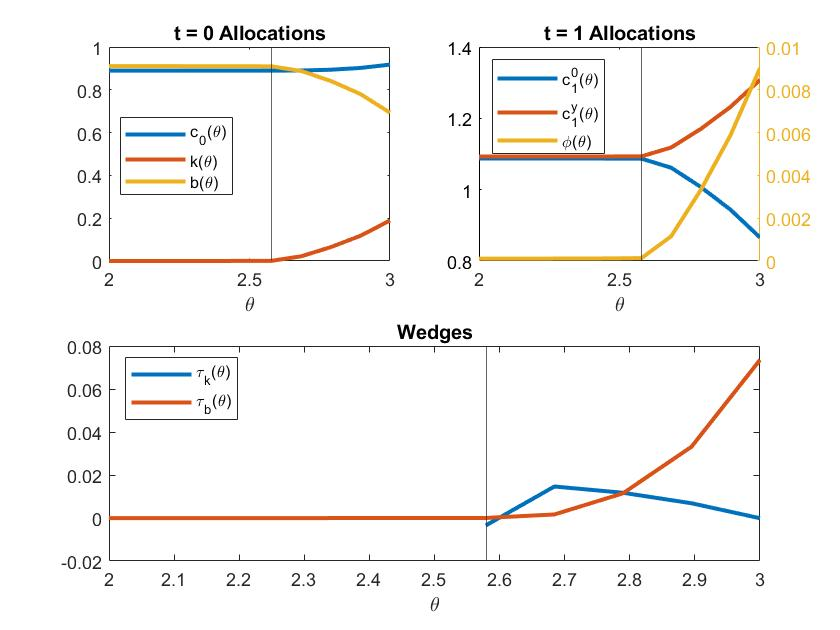
\includegraphics[width = 0.9\columnwidth]{figures/allocs_rlow.jpg}
    \end{figure}

\end{frame}

\section{Dynamic Model}

\begin{frame}
    \frametitle{Dynamic Model: Setup and Timing}

    \begin{itemize}
        \item Static model cannot differentiate between capital income and wealth 
        \item We consider a dynamic extension of the model in order to study wealth accumulation
        \item Time is again discrete, \( t=0,1,... \)
        \item Agents draw new type \( \theta_t \) in each period
        \begin{itemize}
            \item We assume that draws are \textit{i.i.d.}
            \item This way, promised utility is a sufficient statistic for keeping track of history
        \end{itemize}
    \end{itemize}

\end{frame}

\begin{frame}
    \frametitle{Dynamic Model: Setup and Timing}

    Each period plays out as follows:
    \begin{enumerate}
        \item Agents realize their capital income \( y_t \) according to 
        \begin{equation} \label{eqn:dyn_yt}
            y_{t}=\begin{cases}
                \theta_{t-1}k_{t} & \text{with probability }\alpha\\
                0 & \text{with probability } 1-\alpha
                \end{cases}
        \end{equation}
        \item Agents draw new type \( \theta_t \) from \( F\left( \theta \right) \)
        \item Agents make consumption and savings choices \( c_{t}\left(\theta^{t},y^{t}\right),k_{t+1}\left(\theta^{t},y^{t}\right) \), and \( b_{t+1}\left(\theta^{t},y^{t}\right) \)
        \begin{itemize}
            \item Superscript notation denotes history, e.g. \( y^t = \left\{ y_0, y_1,...,y_t\right\} \)
        \end{itemize}
    \end{enumerate}

\end{frame}

\begin{frame}
    \frametitle{Dynamic Model: Dual Planner's Problem}

    \begin{itemize}
        \item \( \mu_t\left( \theta^t, y^t \right) \): measure of period-\( t \) histories induced by the stochastic process governing \( \theta_t \) and the random nature in \( y_t \)
        \item Promised utility:
        \begin{multline*}
            w_{t+1}\left(\theta^{t},y^{t+1}\right)=\\
            \sum_{s=t+1}^{\infty}\beta^{s-t-1}\int u\left(c_{s}\left(\theta^{s},y^{s}\right)\right)d\mu_{s}\left(\theta^{s},y^{s}|\theta^{t},y^{t+1}\right)
        \end{multline*}
        allocated to agent with history \( \left( \theta^t,y^t \right) \), conditional on realization of \( y_{t+1} \)
        \item  We consider the dual planner's problem: minimize the time-0 discounted cost of delivering total utility \( w \)
    \end{itemize}

\end{frame}

\begin{frame}
    \frametitle{Dynamic Model: Dual Planner's Problem} % appendix?

    Recursive formulation:
    \begin{multline}
        C\left(w\right)= \min_{c,k',w_{y}^{\prime},w_{0}^{\prime},\mathcal{U}} \\
        \int\left\{ c\left(\theta\right)-\frac{\alpha\theta k\left(\theta\right)}{R}+R^{-1}\left[\alpha C\left(w_{y}^{\prime}\left(\theta\right)\right)+\left(1-\alpha\right)C\left(w_{0}'\left(\theta\right)\right)\right]\right\} dF\left(\theta\right) \\ \label{eqn:plan_rec}
    \end{multline}
    subject to 
    \begin{align*}
        \int\mathcal{U}\left(\theta\right)dF\left(\theta\right) &\ge w \\
        \mathcal{U}\left(\theta\right) &= u\left(c\right)+\beta\left[\alpha w_{y}^{\prime}\left(\theta\right)+\left(1-\alpha\right)w_{0}^{\prime}\left(\theta\right)\right]  \\
        \mathcal{U}^{\prime}\left(\theta\right) &= u^{\prime}\left(c\right)\frac{k}{\theta}  \\
        \mathcal{U}\left(\underline{\theta}\right) &\ge u\left(c+k\right)+\beta w_{0}^{\prime} 
    \end{align*}
    

\end{frame}

\begin{frame}
    \frametitle{Dynamic Model: Closed-form solution}

    \begin{block}{Proposition 3: Solution to the Dynamic Model}
        If \( u\left( c \right) = \log c \), then \eqref{eqn:plan_rec} admits the following closed-form solution:
        \begin{align*}
            C(w) &= A\exp\left( \left(1-\beta\right)w \right) &
            w^{\prime}\left(\theta,0,w\right)&=w^{\prime}\left(\theta,0\right)+w \\
            k\left(\theta,w\right)&=k\left(\theta\right)\exp\left(\left(1-\beta\right)w\right) & 
            w^{\prime}\left(\theta,y,w\right)&=w^{\prime}\left(\theta,y\right)+w \\
            c\left(\theta,w\right)&=c\left(\theta\right)\exp\left(\left(1-\beta\right)w\right) &
            \mathcal{U}\left(\theta,w\right)&=\mathcal{U}\left(\theta\right)+w
        \end{align*}
        for some \( A,c\left(\theta\right),k\left(\theta\right),w^{\prime}\left(\theta,y\right),w^{\prime}\left(\theta,0\right) \), and \( \mathcal{U}\left( \theta \right) \). 
    \end{block}
    \begin{itemize}
        \item A similar result holds if utility is CRRA with \( \sigma\ne 1 \).
    \end{itemize}
\end{frame}

\begin{frame}
    \frametitle{Dynamic Model: Wedges}

    \begin{itemize}
        \item Proposition 3 shows that wedges in the planner's cost minimization problem are \textit{history-independent}.
        \item Instead, the wedges only depend on the pair \( \theta_t,\theta_{t+1} \)
        \item For example, the wedge on risky investment is given by 
        \begin{align*}
            \tau_{t,k}\left(\theta^{t},y^{t}\right)&=1-\frac{u^{\prime}\left(c_{t}\left(\theta^{t},y^{t}\right)\right)}{\alpha\beta\theta_{t}u^{\prime}\left(c_{t+1}\left(\theta^{t+1},\left\{ y^{t},y\right\} \right)\right)} \\
            &= 1-\frac{1/c\left(\theta_{t}\right)}{\alpha\beta\theta_{t}\left\{ 1/c\left(\theta_{t+1}\right)\exp\left[\left(1-\beta\right)w_{t+1}^{y}\left(\theta_{t}\right)\right]\right\} }
        \end{align*}
    \end{itemize}

\end{frame}

\begin{frame}
    \frametitle{Implementation}

    \begin{itemize}
        \item Thus far, we have focused on optimal \textit{wedges} in the mechanism design problem
        \item The question remains: how to implement these wedges with taxes and transfers in a competitive market economy?
    \end{itemize}

\end{frame}

\begin{frame}
    \frametitle{Implementation: Wealth Subsidy}

    \begin{itemize}
        \item The lack of history-dependence in the solution to the dynamic planner's problem makes implementation somewhat difficult
        \item At the optimum, we need two individuals with different histories but the same current and one period-ahead types to face identical distortions 
        \item If we want to implement a progressive tax on capital income, then to accomplish this result, we would need to pair this tax with a wealth \textit{subsidy}
        \begin{itemize}
            \item Progressive tax would need to be ``undone'' to preserve history independence
        \end{itemize}
    \end{itemize}

\end{frame}

\section{Conclusion}

\begin{frame}
    \frametitle{Conclusion}

    \begin{itemize}
        \item We have studied optimal taxation of capital income in an environment with informational frictions
        \item Static model: positive wedge on risk-free savings, non-monotonic marginal subsidies on capital income for entrepreneurs 
        \begin{itemize}
            \item No distortions for workers, or ``lenders''
        \end{itemize}
        \item Dynamic model: with i.i.d. productivity shocks, optimal wedges are history-independent
    \end{itemize}

\end{frame}

\begin{frame}
    \frametitle{Next Steps}

    \begin{itemize}
        \item Full solution to static model 
        \item Characterization of history-independent wedges 
        \item Dynamic model: persistence in \( \theta \)
        \begin{itemize}
            \item Less tractable, but perhaps more intuitive
        \end{itemize}
        \item Implementation: construct a tax-and-transfer system that generates the optimal allocations as a competitive equilibrium 
    \end{itemize}

\end{frame}

\begin{frame}[allowframebreaks]
    \frametitle{References}

    \bibliographystyle{named}
    \bibliography{summer_paper}

\end{frame}
\end{document}